\documentclass[9pt,reqno]{amsart}
\usepackage{graphicx}
% \usepackage[a4paper, total={5.5in, 8in}]{geometry}
%\usepackage{mathpazo}
%\usepackage{euler}


\graphicspath{ {./urpimages/} }
\usepackage{amsfonts,amssymb,latexsym,amsmath, amsthm}
\usepackage{tikz-cd}
\usepackage{mathrsfs}
\usepackage{stmaryrd}
\usepackage{hyperref}
\hypersetup{
    colorlinks = true,
    linkbordercolor = {red}
}
\theoremstyle{definition}
%% this allows for theorems which are not automatically numbered
\newtheorem{defi}{Definition}[section]
\newtheorem{theorem}{Theorem}[section]
\newtheorem{lemma}{Lemma}[section]
\newtheorem{obs}{Observation}
\newtheorem{exercise}{Exercise}[section]
\newtheorem{rem}{Remark}[section]
\newtheorem{construction}{Construction}[section]
\newtheorem{prop}{Proposition}[section]
\newtheorem{coro}{Corollary}[section]
\newtheorem{disc}{Discussion}[section]
\DeclareMathOperator{\spec}{Spec}
\DeclareMathOperator{\im}{im}
\DeclareMathOperator{\obj}{obj}
\DeclareMathOperator{\ext}{Ext}
\DeclareMathOperator{\tor}{Tor}
\DeclareMathOperator{\ann}{ann}
\DeclareMathOperator{\id}{id}
\DeclareMathOperator{\proj}{Proj}
\DeclareMathOperator{\gal}{Gal}
\DeclareMathOperator{\coker}{coker}
\newcommand{\degg}{\textup{deg}}
\newtheorem{ex}{Example}[section]
%% The above lines are for formatting.  In general, you will not want to change these.
%%Commands to make life easier
\newcommand{\RR}{\mathbf R}
\newcommand{\aff}{\mathbf A}
\newcommand{\ff}{\mathbf F}
\usepackage{mathtools}
\newcommand{\cccC}{\mathbf C}
\newcommand{\oo}{\mathcal{O}}
% \newcommand{\ZZ}{\mathbf Z}
\newcommand{\pring}{k[x_1, \ldots , x_n]}
\newcommand{\polyring}{[x_1, \ldots , x_n]}
\newcommand{\poly}{\sum_{\alpha} a_{\alpha} x^{\alpha}} 
\newcommand{\ZZn}[1]{\ZZ/{#1}\ZZ}
% \newcommand{\QQ}{\mathbf Q}
\newcommand{\rr}{\mathbf R}
\newcommand{\cc}{\mathbf C}
\newcommand{\complex}{\mathbf {C}_\bullet}
\newcommand{\nn}{\mathbf N}
\newcommand{\zz}{\mathbf Z}
\newcommand{\PP}{\mathbf P}
\newcommand{\cat}{\mathbf{C}}
\newcommand{\ca}{\mathbf}
\newcommand{\zzn}[1]{\zz/{#1}\zz}
\newcommand{\qq}{\mathbf Q}
\newcommand{\calM}{\mathcal M}
\newcommand{\latex}{\LaTeX}
\newcommand{\V}{\mathbf V}
\newcommand{\tex}{\TeX}
\newcommand{\sm}{\setminus} 
\newcommand{\dom}{\text{Dom}}
\newcommand{\lcm}{\text{lcm}}
\DeclareMathOperator{\GL}{GL}
\DeclareMathOperator{\Hom}{Hom}
\DeclareMathOperator{\aut}{Aut}
\DeclareMathOperator{\SL}{SL}
\DeclareMathOperator{\inn}{Inn}
\DeclareMathOperator{\card}{card}
\newcommand{\sym}{\text{Sym}}
\newcommand{\ord}{\text{ord}}
\newcommand{\ran}{\text{Ran}}
\newcommand{\pp}{\prime}
\newcommand{\lra}{\longrightarrow} 
\newcommand{\lmt}{\longmapsto} 
\newcommand{\xlra}{\xlongrightarrow} 
\newcommand{\gap}{\; \; \;}
\newcommand{\Mod}[1]{\ (\mathrm{mod}\ #1)}
\newcommand{\p}{\mathfrak{p}} 
\newcommand{\rmod}{\textit{R}-\textbf{Mod}}
\newcommand{\idealP}{\mathfrak{P}}
\newcommand{\ideala}{\mathfrak{a}}
\newcommand{\idealb}{\mathfrak{b}}
\newcommand{\idealA}{\mathfrak{A}}
\newcommand{\idealB}{\mathfrak{B}}
\newcommand{\X}{\mathfrak{X}}
\newcommand{\idealF}{\mathfrak{F}}
\newcommand{\idealm}{\mathfrak{m}}
\newcommand{\s}{\mathcal{S}}
\newcommand{\cha}{\text{char}}
\newcommand{\ccc}{\mathfrak{C}}
\newcommand{\idealM}{\mathfrak{M}}
\usetikzlibrary{decorations.pathmorphing} 
\newcommand{\overbar}[1]{\mkern 1.5mu\overline{\mkern-1.5mu#1\mkern-1.5mu}\mkern 1.5mu}

%Itemize gap:

% \pagecolor{black}
% \color{white}
% Author info

\title{Math 425A HW4, Due 09/23/2022, 6PM}
\author{Juan Serratos}
\email{jserrato@usc.edu}
\date{ September 17, 2022 \\ {Department of Mathematics, University of Southern California}}
\address{Department of Mathematics, University of Southern California, 
Los Angeles, CA 90007}
\begin{document}
\maketitle
\setcounter{tocdepth}{4}
\setcounter{secnumdepth}{4}

\section*{Chapter 2. \S 5.}
\begin{exercise}[5.2.] Let $a_1, a_2, \ldots$ be any enumeration of the negative rational numbers; let $b_1, b_2, \ldots$ be any enumeration of the positive rational numbers. Show that the following two equalities hold:
\[
\bigcap^\infty_{j=1} (a_j, b_j) = \{ 0 \}, \bigcup_{j=1}^\infty (a_j, b_j) = \rr
\]
\end{exercise}
\begin{proof} WLOG, for the first equality, it will suffice to show that $\bigcap^\infty_{j=1} (a_j, b_j)  \subseteq \{ 0 \}$. Take $\ell \in T = \bigcap^\infty_{j=1} (a_j, b_j)$. Then $a_j < \ell < b_j$ for every $ j \geq 1$. Now we can find some $\epsilon > 0$ with $b_j < \epsilon$. As $\ell < b_j$ then we have that $ \ell < \epsilon$, and as $\epsilon > 0$, then $\ell \leq 0$. Similarly, we can find some $\epsilon < 0$  (i.e. $0>-\epsilon$) with $a_j > - \epsilon$. So then as $\ell > a_j$, $0>a_j > -\epsilon$, and $\epsilon >0$, then we must have that $\ell \geq 0$. Thus, all together, we have that $0 \leq \ell \leq 0$, and hence we have that $\ell = 0$.

For the second equality, it suffices to show WLOG that $ \rr \subseteq \bigcup_{j=1}^\infty (a_j, b_j )$. Suppose have that $\ell \in \rr$ and $\ell >0$---if $\ell =0$ then the result is clear. Then $\ell +1 > \ell$ and so there is some $s \in (\ell, \ell +1)$; we will write $s = b_j$ for $j \geq 1$. As $\ell >0$, then there is some $t \in (0,\ell )$; we will write $t = b_j$ for some $j \geq 1$. So then $0<a_j < \ell < b_j <\ell +1$, and hence $\ell \in (a_j, b_j)$. Thus $\ell \in \bigcup_{j=1}^\infty (a_j,b_j)$. Now, for the other case, suppose $ \ell < 0$. Then $\ell -1 < \ell$, and so we can find some $q \in (\ell -1, \ell)$; we write $q = a_j$ for some $j \geq 1$. So as $x<0$ then we can find some $p \in (x,0)$; we will write $p = b_j$ for some $j \geq 1$. All together, we have that $\ell -1 <a_j < \ell <b_j <0$. Thus $\ell  \in (a_j, b_j)$ and hence $\ell \in \bigcup_{j=1}^\infty (a_j, b_j)$. Therefore, as $\ell$ was chosen to be simply some random real number, then $\bigcup_{j=1}^\infty (a_j, b_j) = \rr$.
\end{proof}
\section*{Chapter 2. $\S$ 6.}
\begin{exercise}[6.1.] Prove that the addition and multiplication operations in $(\cc, + ,\cdot)$ satisfy the field axioms of Definition 2.1.
\end{exercise}
\begin{proof}
	We essentially need to show that five axioms hold true from Definition 2.1. From now on, let $x, y, z \in \rr \times \rr \, (=\cc)$, which is the underlying set of $\cc$, where $x = (a, b), y = (c,d), z = (s,t)$ where $a,b,c,d,s,t \in \rr$.
	
	(1) The set $\cc :=(\cc, +, \cdot)$, as the operations are defined in Chapter $2, \S 6$., is closed since $x+y = (a,b) + (c,d) = (a+c, b+d) \in \rr \times \rr$ and $xy = (a, b) \cdot (c,d) = (ac-bd, ad+bc) \in \rr \times \rr$ since $a+c , b+d, ac-bd, ad+bc  \in \rr$ as $\rr$ is a field, and so $x+y \in \cc$ and $xy \in \cc$.
	
	(2) For commutativity: $x+y = (a,b) + (c,d) = (a+c, b+d) = (c+a, d+b) = (c,d )+(a,b) = y+x$ since $\rr$ is a field, and, similarly, $xy = (a, b) \cdot (c,d) = (ac-bd, ad+bc) = (ca-db, cb+da) = (c,d) \cdot (a,b) = yx$ as $\rr$ is a field. Now for associativity:
	\begin{align*}
		x+(y+z) &= (a, b) + ((c,d)+(s,t)) = (a,b) + (c+s, d+t) \\
		&= (a+(c+s), b+(d+t)) = ((a+c)+s, (b+d)+t)) && ( \rr \text{ is a field} )\\
		&= (a+c, b+d) + (s, t)= (x+y)+z
	\end{align*}
	\begin{align*}
		x(yz)& =(a,b) \cdot ((c,d)\cdot (s,t)) = (a,b)\cdot (cs -dt, ct+ds) \\ &= (a(cs-dt)-b(ct+ds), a(ct+ds)+b(cs-dt)) && ( \rr \text{ is a field} ) \\ 
		&= (acs-adt-bct-bds, act+ads+bcs-bdt) && ( \rr \text{ is a field} ) \\ &= ((ac-bd)s-(ad+bc)t, (ad+bc)s+(ac-bd)t) && ( \rr \text{ is a field} )\\ &= (ac-bd, ad+bc) \cdot (s, t) = ((a,b) \cdot (c,d)) \cdot (s,t) \\
			&= (xy)z
	\end{align*} Therefore we have associativity and commutativity with the defined operations on $\cc$. 
	

	(3) The additive identity of $\cc$ is defined to be $0 = (0, 0) \in \rr \times \rr$, and so $x+0 = (a,b) +(0,0)= (a+0, b+0) = (a,b) = (0+a, 0+b) = (0, 0) + (a,b) = 0 +x$. Similarly, the multiplicative identity is defined to be $1 =(1, 0)$, and so $x \cdot 1 = (a,b) \cdot(1,0) = (a(1)-b(0), a(0)+b(1)) = (a, b) = x = 1 \cdot x = (1, 0) \cdot (a,b) = (1(a) - 0(b), 1(b)+0(a)) = (a,b) = x$.
	
	(4) The multiplicative inverse of $x = (a,b)$, where $x \neq 0$, can be found to be \\ $x^{-1} = \left (\frac{a}{a^2+b^2}, \frac{-b(\frac{a}{a^2+b^2})}{a} \right)$, and we can tediously calculate to get that 
	\begin{align}
	x \cdot x^{-1} = (a,b) \cdot \left (\frac{a}{a^2+b^2}, \frac{-b(\frac{a}{a^2+b^2})}{a} \right ) = \left (\frac{a}{a^2+b^2}, \frac{-b}{a^2+b^2} \right ) =(1,0) = 1.
	\end{align} The additive inverse is much easier: for $y = (c,d)$, the additive inverse is $ -y = (-c, -d)$, and so $y+(-y) = (c+(-c), d+(-d)) = (0, 0) = 0$. 
	
	(5) Lastly, we need to check distributivity: Let $t := y+z = (c+s, d+t)$. Now 
	\begin{align*}
x \cdot t = (a,b) \cdot (c+s, d+t) &= (a(c+s)-b(d+t), a(d+t)+b(c+s)) \\ &= (ac+as-bd-bt, ad+at+bc+bs) \\
&= ((ac-bd)+(as-bt) , (ad+bc) + (at+bs)) \\
&= (a,b) \cdot (c,d) + (a,b) \cdot (s,t)
	\end{align*}
Therefore the distributive law holds.

Hence $\cc$ is indeed a field. 
\end{proof}
\begin{exercise}[6.2.] Prove that there exists no order $\leq$ that makes $(\cc, +, \cdot,  \leq)$ into an ordered field. (Hint: If there were such an ordering, then $i = \sqrt{-1}$ would necessarily be either positive or negative.)
\end{exercise}
\begin{proof}
	Suppose that there does exists an ordering that makes $\cc$ into an ordered field. Then, by definition, we have that either $i \leq 0$ or $i \leq 0$, but we do not have that $i = 0$, so we simply have that either $i$ is negative or positive. Suppose, for the first case, that $i<0$. Then $0 < -i$ so $0^2 <(-i)^2 = 1(-1) = -1$ and once again, $0^2 < (-1)^2 = 1$; hence a contradiction. Thus we cannot have that $i$ is negative. Now, for the second/last case, then assume that $i>0$. Then $i^2 = -1 >0^2 = 0$ and so $(-1)+1 =0> 0 +1 =1$, and multiplying by $1$, $i \cdot 0 = 0 > 1 \cdot i = i$; thus a contradiction. Hence we cannot have that $i$ is not positive either. Therefore we cannot have that there exists an order on $\cc$ that makes it into an ordered field. 
	\end{proof}

\section{Chapter 3. $\S$ 1}
\begin{exercise}[1.1.] Let $\| \cdot \|$ be a norm on a real vector space $V$. Prove the \textit{reverse triangle inequality:}
\[ | \|x \| - \|y \| | \leq  \| x-y \| 
\]
\end{exercise}
\begin{proof}
	Firstly, as we have that $\| \cdot \|$ is a norm, then: $\|x-y\| = \|-(y-x)\| = |-1| \|y-x\| = \|y-x\|$. Now $\|x \| = \|(x-y) + y \| \leq \|x-y \| + \|y\| $, and so $\|x\|- \|y\| \leq \|x-y\|$. Similarly, $\|y \| = \|(y-x)+x \| \leq \|y-x\| + \|x \|$, so $\|y\|- \|x\| \leq \|y-x\|$, which can be rewritten as $-\|y-x \| \leq \|x\|-\|y\|$. Thus we can write $ - \|y-x\| \leq \|x\|- \|y \| \leq \|x-y\|$. And this can finally be rewritten as $- \|x-y\| \leq \|x\|-\|y\| \leq \|x-y\|$. Hence $\left | \|x\|-\|y\| \right| \leq \|x-y\|$. 
\end{proof}
\begin{exercise}[1.2.] Prove that any complex inner product is conjugate linear in its second argument; that is,
\[ \langle x, \lambda y + z \rangle = \overline{\lambda}\langle x, y \rangle + \langle x, z \rangle ,
\] for any scalar $\lambda$. (Note that this implies that any real inner product is linear in its second argument.)
\end{exercise}
\begin{proof} We are considering a complex inner product and so we have a mapping $\langle \cdot, \cdot \rangle \colon V\times V \to \cc$ with some properties. Let $x, y, z \in V$ and $\lambda \in \cc$. Then $\langle x, \lambda y+z \rangle = \overline{\langle \lambda y+z, x \rangle} = \overline{\lambda \langle y, x \rangle} + \overline {\langle z, x\rangle} = ( \overline{ \lambda } ) \overline{\langle y, x \rangle} + \overline{\langle z, x\rangle} = \overline{\lambda} \langle x,y\rangle + \langle x, z \rangle$. 
\end{proof}
\begin{exercise}[1.3.-Polarization identity]  If $(V, \langle \cdot, \cdot \rangle)$ is a real inner product space, then 
\[ \langle v, w \rangle = \frac{1}{4} \left [ \| v+w \|^2 - \|v - w \|^2 \right ], \; \text{for all $v, w \in V$.}
\]
If $(V, \langle \cdot, \cdot \rangle )$ is a complex inner product space, then 

\[ 
\langle v , w \rangle = \frac{1}{4} \left [ ( \|v + w \|^2 - \|v - w \|^2) + i( \| v + i w \|^2 - \|v-iw\|^2) \right] 
\] 
	
\end{exercise}
\begin{proof}
	Suppose that $(V, \langle \cdot, \cdot \rangle)$ is a real inner product space. Then $\| v+w \|^2 = \langle v+w, v+w \rangle = \langle v,v \rangle + \langle v,w \rangle + \langle w, v \rangle + \langle w, w \rangle = \langle v,v \rangle + 2 \langle v,w \rangle  + \langle w, w \rangle$, and, similarly, $\| v-w\|^2 = \langle v-w, v-w \rangle= \langle v,v \rangle -\langle v,w \rangle - \langle w, v \rangle + \langle w, w \rangle = \langle v,v \rangle - 2\langle v,w \rangle + \langle w, w \rangle$. Thus: 
\begin{align*}
	\frac{1}{4} \left [ \| v+w \|^2 - \|v - w \|^2 \right ] &= \frac{1}{4} \left[ \langle v,v \rangle + 2 \langle v,w \rangle  + \langle w, w \rangle - (\langle v,v \rangle - 2\langle v,w \rangle + \langle w, w \rangle ) \right] \\ 
	&= \frac{1}{4} \left[ 2\langle v, w \rangle + 2 \langle v, w \rangle \right]\\
	&= \frac{1}{4} \left[4 \langle v, w \rangle \right] = \langle v,w \rangle.
\end{align*}

Suppose that $(V, \langle \cdot, \cdot \rangle$) is a complex inner product. Similar to the first computations we did for the real case, we can find that $\|v+w\|^2 = \langle v, v \rangle = \langle v, w \rangle  + \overline{\langle v, w \rangle } + \langle w, w \rangle $, and $\|v -w \|^2 = \langle v,v \rangle - \langle v,w \rangle - \overline{\langle v, w \rangle }+ \langle w, w \rangle $. Moreover, $\|v+iw\| = \langle w, w \rangle + i \langle w, v \rangle -i\langle v, w\rangle + \langle v, v \rangle $, and $\|v-iw \|= \langle w,w \rangle -i \langle w, v \rangle + i \langle v, w \rangle + \langle v, v \rangle $. Now:
\begin{align*}
	\|v+w \|^2-\|v-w\|^2 &= 2 \langle v,w \rangle +2 \langle w,v \rangle, \; \text{and} \\
	\|v+iw\|^2-\|v-iw\|^2 &= 2i \langle w,v \rangle -2i \langle v,w \rangle = 2i \left [ \langle w,v \rangle - \langle v, w \rangle \right] 
\end{align*}
Thus: 
\begin{align*}
	\frac{1}{4} \left [ \left ( 2 \langle v,w \rangle +2 \langle w,v \rangle \right ) + i \left (2i (\langle w,v \rangle - \langle v, w \rangle \right) \right ] &= \frac{1}{4} \left [ 2 \langle v,w \rangle +2 \langle w,v \rangle +  (-2 \langle w,v \rangle +2 \langle v, w \rangle ) \right ]\\
	&= \frac{1}{4}\left[ 4 \langle v,w \rangle + 2 \langle w, v \rangle -2\langle w , v\rangle \right]\\
	&= \frac{1}{4} \left[4 \langle v, w \rangle \right] = \langle v, w \rangle.
	\end{align*}
\end{proof}
\section{Chapter 3 \S 2}
\begin{exercise}[2.2]
	 For each of $(a)$, $(b)$, and $(c)$, determine whether the given function $d_j$ is a metric on $\rr$, and prove that your answer is correct.
	 \begin{itemize}
	 	\item [(a)] $d_1 (x, y) = \sqrt{ |x-y|}$
	 	\item [(b)] $d_2 (x, y) = |x-2y|$.
	 	\item [(c)] $d_3 (x, y) = \frac{|x-y|}{1+|x-y|}$
	 \end{itemize}
\end{exercise}
\begin{proof}
	(a) Indeed a metric. We need to show that $d_1 \colon X \times X \to \rr$  satisfies nonnegativity, symmetry, and the triangle inequality:
	
	 Firstly, let's fix some arbitrary $(x,y) \in X \times X$. Then $d_1(x,y) = \sqrt{|x-y|}$, which is the root of some positive number, or $0$, in $\rr$, and so $d_1(x,y) \geq 0$; if $x =y$, then $\sqrt{|x-y|} = \sqrt{|x-x|} = 0$, and if we first assumed $d_1(x,y)= 0$, then $d_1(x,y) = \sqrt{|x-y|} = 0$ and so $|x-y| = 0$ and in either case of $x-y\geq 0$ or $x-y < 0$, we get that $x=y$. 
	 
	 For symmetry, suppose we have $d_1(x,y)$ and $(x,y) \in X \times X$. Now, consider $d_1(x,y) - d_1(y,x)$, and so $\sqrt{|x-y|} - \sqrt{|y-x|}$---if $x-y>0$ then $0 >y-x$, which implies $\sqrt{x-y} - \sqrt{-(y-x)}  = \sqrt{x-y} - \sqrt{x-y} = 0$ and so $d_1(x,y) = d_1(y,x)$ if $x-y>0$; if $x-y<0$ then $0<y-x$, so $\sqrt{-(x-y)} - \sqrt{y-x} = \sqrt{y-x} - \sqrt{y-x} = 0$ and so $d_1(x,y) = d_1 (y,x)$ if $x-y<0$; if $x-y = 0$ then $x=y$ and $d_1(x,y) = \sqrt{|x-y|} = \sqrt{|y-x}| = d_2(y,x)$. Thus $d_1$ is symmetric. [Could use instead the fact that $| \cdot |$ is a metric, and so $ (d_1(x,y))^2 = |x-y| = |y-x| = (d_1(y,x))^2$, and so $d_1(x,y) = d_1(y,x)$.]
	 
	 Lastly, we need to show that the triangle inequality holds. This is shown easiest if we show that, for any $s, t \in \rr$ such that $s,t \geq 0$, we have that $\sqrt{s}+\sqrt{t} \geq \sqrt{s+t}$. This is true as we clearly have that $2\sqrt{st} \geq 0$ and so this leads to $s+\sqrt{2st} + t  \geq s+t$ which is the same as $(\sqrt{s}+\sqrt{t})^2 \geq s+t$, and thus $\sqrt{s}+\sqrt{t} \geq \sqrt{s+t}$. Now, $d_1(x,y) = \sqrt{|x-y|} = \sqrt{|(x-z)+(z-y)|} \leq \sqrt{|x-z|} + \sqrt{|z-y|} = d_1(x,z) +d_1(z,y)$---note that if $x-y<0$ then the inequality would still work out in the end.    
	 
	 Therefore we have that $d_1 \colon X \times X \to \rr$ where $d_1 \colon (x,y) \mapsto \sqrt{|x-y|}$ does define a metric. 

	(b) $d_2(x,y) = |x-2y|$ does not define a metric on $\rr$, since it does not, at the very least, satisfy the symmetry condition: Let $X = \rr$. Then $d_2 \colon \rr \times \rr \to \rr$, where $d_2 \colon (x,y) \mapsto |x-2y|$, is not a metric since, for example, $d_2(2, 3) = |2-2(3)| = |2-6| = |-4| = 4$ but $d_2(3,2) = |3-2(2)| = |3-4| = |-1| = 1$, and so a counter example against the symmetry property.  
	
	(c) Indeed a metric.
	
	Suppose $(x,y) \in X \times X$. Then $\frac{|x-y|}{1+|x-y|}$ is always positive since $|x-y| \geq 1$ for any choice $x \neq y$ and $x=y$ gives us that $d_3(x,y) = 0$. Now if $x=y$, then $\frac{0}{1+0} = 0$. If instead assumed firstly that $\frac{|x-y|}{1+|x-y|} = 0$, then: $x-y>0$ implies $\frac{x-y}{1+x-y} = 0$ and so $x=y$ clearly, and similarly, $x-y<0$ gives us $\frac{y-x}{1+y-x} = 0 $ and so $x=y$; if $x -y = 0$, then the result follows immediately. Thus $d_3(x,y) \geq 0$ for all $x,y \in X$ and $d_3(x,y) = 0$ if and only if $x =y$.
	
	For symmetry, we proceed as follows. If $x-y = 0$ then the result is clear. Now if $x-y>0$, then 
	\begin{align*}
		\frac{|x-y|}{1+|x-y|} - \frac{|y-x|}{1+|y-x|} &= \frac{x-y}{1+x-y} - \frac{-(y-x)}{1+(-1)(y-x)} \\
		&= \frac{x-y}{1+x-y} + \frac{y-x}{1+(x-y)} = 0.
	\end{align*} Thus $d_1(x,y) = d_1(y,x)$ if $x-y>0$. If $x-y<0$, then
	\begin{align*}
		\frac{|x-y|}{1+|x-y|} - \frac{|y-x|}{1+|y-x|} &= \frac{-(x-y)}{1+(-1)(x-y)} - \frac{y-x}{1+y-x} \\
		&= \frac{y-x}{1+y-x} + \frac{-y+x}{1+y-x} = 0.
	\end{align*} Thus $d_3(x,y) = d_3(y,x)$ if $x-y<0$. Lastly, we have that if $x-y = 0$, then $x=y$, and so, trivially, $d_3(x,y) = d_3(y,x)$. Therefore $d_3$ is symmetric. [It would have been easier to see that, as $|x-y|$ itself defines a metric, then $\frac{|x-y|}{1+|x-y|} = \frac{|y-x|}{1+|y-x|}$, and so $d(x,y) = d(y,x)$.]
	
	For the triangle inequality
	\begin{align*}
		d(x,y) + d(y,z) = \frac{|x-y|}{1+|x-y|} + \frac{|y-z|}{1+|y-z|} &\geq \frac{|x-y|}{1+|x-y|+|y-z|} + \frac{|y-z|}{1+|x-y|+|y-z|} \\ 
		&= \frac{|x-y|+|y-z|}{1+|x-y|+|y-z|}  \\ 
		&= 1-\frac{1}{1+|x-y|+|y-z|} \\
		& \geq 1 - \frac{1}{1+|x-z|} = \frac{1+|x-z|-1}{1+|x-z|} = \frac{|x-z|}{1+|x-z|} = d_3(x,z).
	\end{align*}	
	Therefore the triangle inequality holds and $d_3 \colon X \times X \to \rr$ defines a metric. 
\end{proof}
\begin{exercise}[2.3]
Consider the function $d \colon \rr^2 \times \rr^2 \to \rr$ defined by 
\[ d(x,y) = |x_1 -y_1| + |x_2 -y_2|, \; \; [ \, x = (x_1, x_2), \; y= (y_1, y_2) \, ] 
\] 
\begin{itemize}
	\item [(a)] Prove that $d$ is a metric on $\rr^2$.
	\item [(b)] On a sheet of graph paper, draw the set $B_d ((5,1), 3)$. Use dotted lines to indicate the ‘boundary’, which is not included in the set you are drawing. (Hint: it may be easier to figure out what the set looks like if you first consider $B_d ((0, 0), 3)$.)
	\item [(c)] On the same graph as in the previous part, draw $B_{d_u} ((-3, 2), 1)$, where $d_u$ denotes the square metric.
\end{itemize}
\end{exercise}
\begin{proof}
	(a) We always have that $d(x,y) \geq 0$ since $|\cdot |$ is itself a metric, and so $|x_1 -y_1| \geq 0$ and $|x_2 - y_2 | \geq 0$. Now if $d(x,y) = 0$, then we must have that $|x_1 -y_1| =0$ and $|x_2 - y_2| = 0$, and so we have that $x_1 = y_1 $ and $x_2 = y_2$. Hence $x=y$.
	
	We have that the symmetry property holds as a consequence of the fact that $|\cdot|$ is a metric, and so $d (x,y) = d( (x_1,x_2), (y_1, y_2))= |x_1 -y_1| + |x_2-y_2| = |y_1-x_1 |+|y_2-x_2| = d((y_1, y_2), (x_1, x_2))=d(y,x)$. 
	
	Lastly, let $z= (z_1, z_2) \in \rr^2$. Then using the triangle inequality for the absolute value on $\rr$, then we can show that it works for this metric: $d(x,y) = |x_1 - y_1| + |x_2 -y_2| = |x_1 -z_1 +z_1 -y_1| + |x_2 -z_2 + z_2 -y_2 | \leq |x_1-z_1| + |z_1 -y_1|+|x_2 - z_2| + |z_2 - y_2|= d(x,z) + d(z,y) $.
\end{proof}
	Hence we have that $d \colon \rr^2 \times \rr^2 \to \rr$ defines a metric. 
\newpage
	(b) 
	
	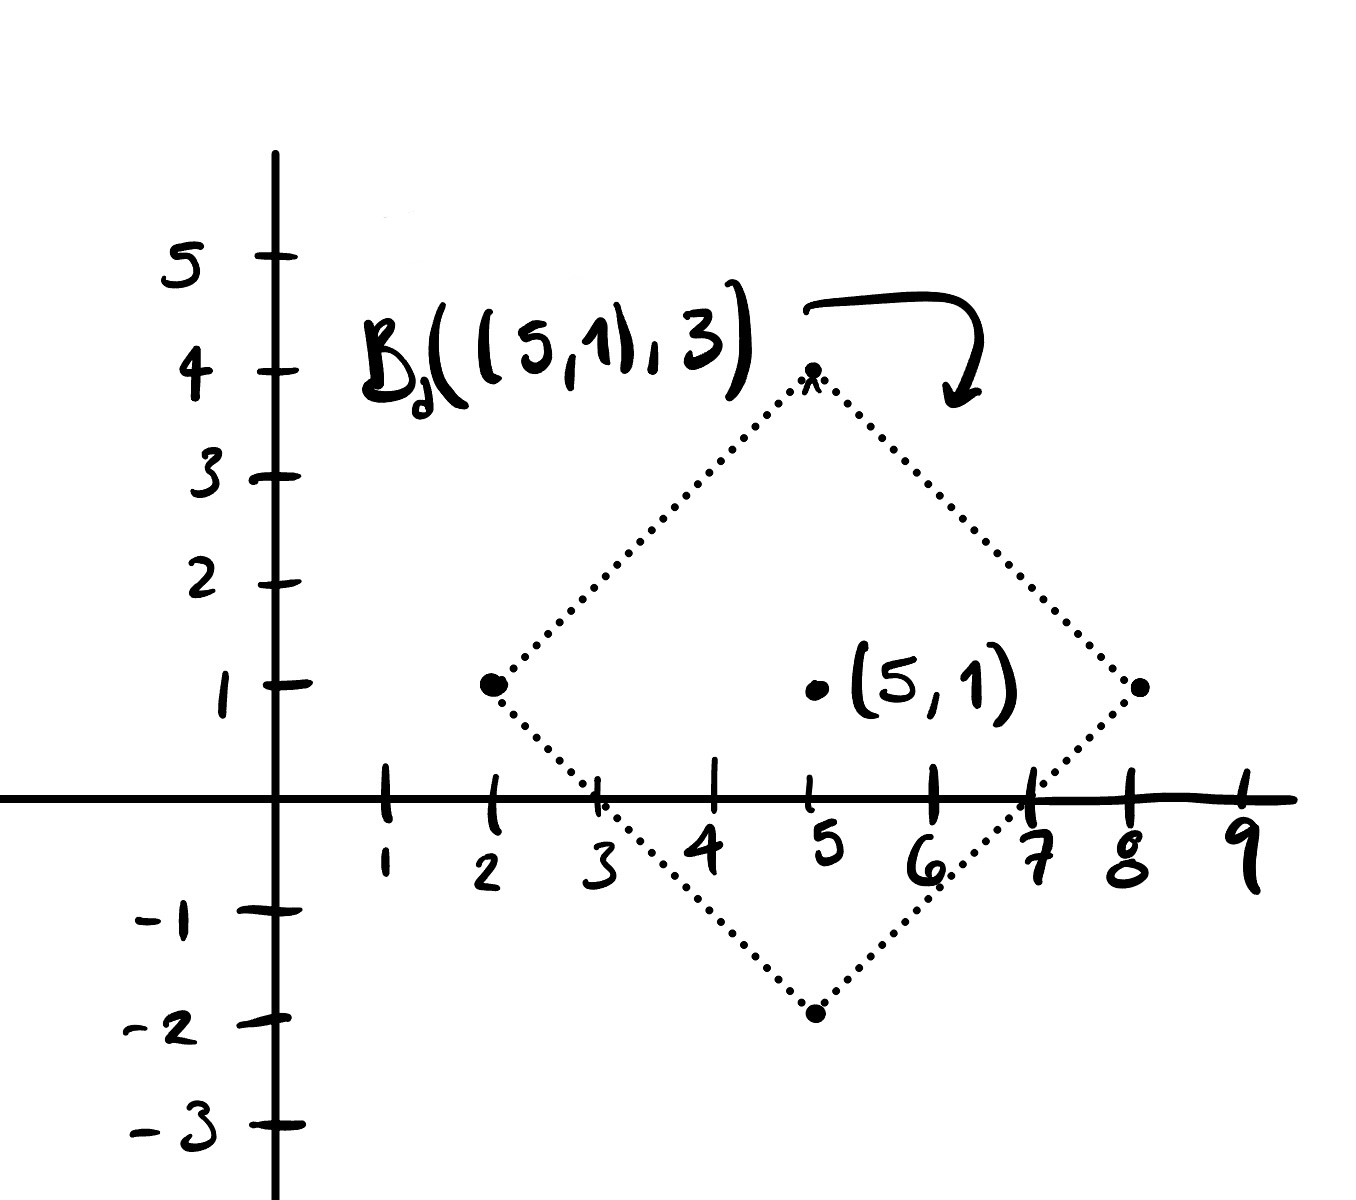
\includegraphics[scale = .2]{IMG_0686.jpg}  
	
	(c) 
	
	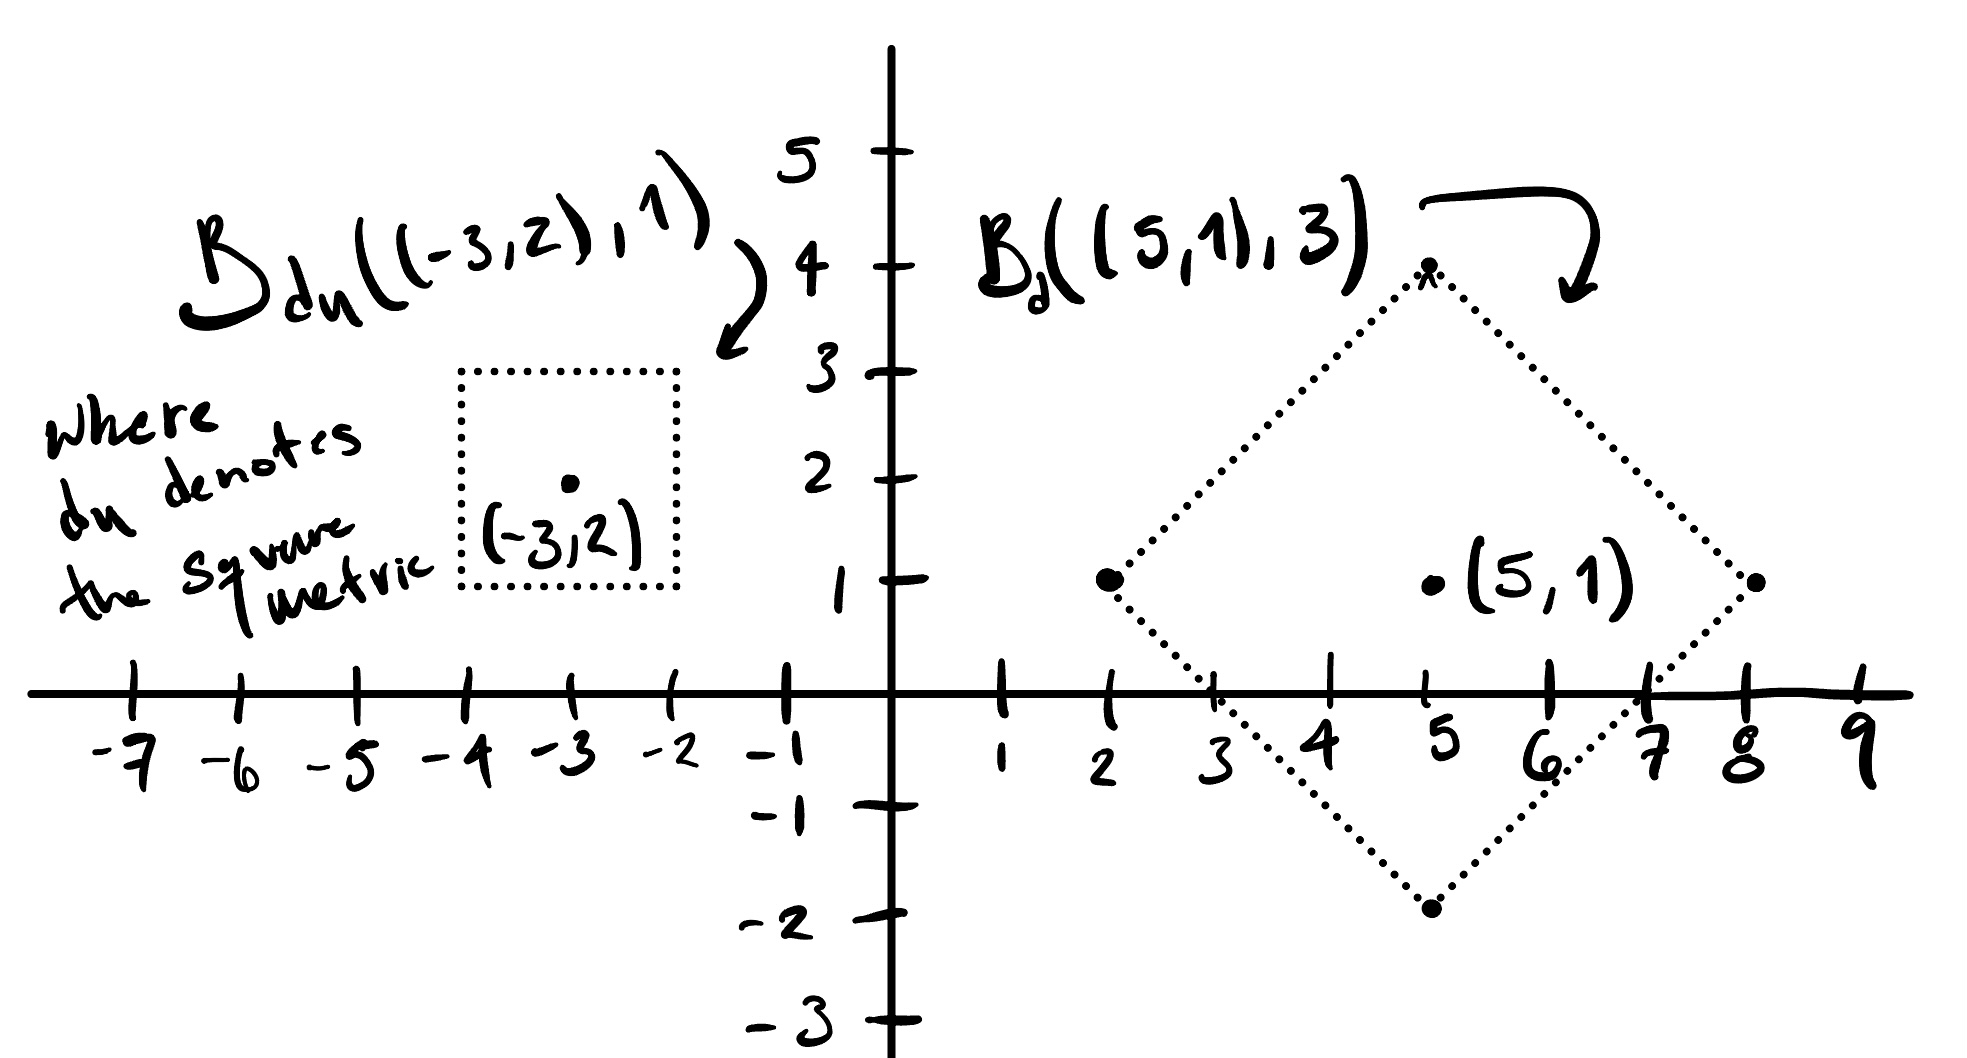
\includegraphics[scale = .2]{IMG_0688.jpg} 
\newpage
\begin{exercise}[2.4.] Let $(X,d)$ be a metric space, and let $E$ be a subset of $X$. The \textit{diameter} of $E$ in $(X,d)$ is defined by the formula 
\[
\text{diam}_d (E) = \sup \{ d(x,y) \colon x,y \in E \}.
\]
\begin{itemize}
	\item[(a)] Prove that for any $r >0$ and $x \in X$, we have $\text{diam} (B(x,r)) \leq 2r$.
	\item[(b)] If $X$ is any set and $d$ is the discrete metric, show that $\text{diam} (B(x, r)) = 0$ for any $r \leq 1$, while $\text{diam} (B(x, r)) = 1$ for any $r > 1$.
	\item[(c)] If $X = \rr^n$ for some $n \in \nn$ and $d$ is the Euclidean metric, prove that $\text{diam} (B(x,r)) = 2r$.
\end{itemize}
\end{exercise}
\begin{proof}
	(a) Suppose that $r>0$ and $x \in X$. Then $\text{diam} (B(x,r)) = \sup \{d(s,t) \colon s,t \in B(x,r) \}$. By definition of the set, without talking about the least upper bound, we're considering real numbers $d(q,p)$ where $q,p \in B (x,r)$, and so $d(x,q) <r$ and $d(x, p ) <r$. Thus $d(q,p) \leq d(q,x) + d(x, p) < 2r$. And so the distance between all points is less than $2r$, i.e. $2r$ is an upper bound for the set. Thus, by the definition of the least upper bound, we have that $\sup \{d(s,t) \colon s,t \in B(x,r) \} \leq 2r$; that is, $\text{diam} (B(x,r)) \leq 2r$.
	
	(b) Suppose $X$ is a set and $d$ is the discrete metric and let $ r \leq 1$. Now $B (x,r) = \{ y \in X \colon d(x,y) < r \}$, but as we assumed $ r \leq 1$, then $B (x,r) = \{ x \}$ itself since we're using the discrete metric. Thus $\sup \{ d(s,t) \colon s,t \in B(x,r) \} = \sup \{ d(x,x) = 0 \} = \sup {0} = 0$. Thus $\text{diam} (B(x,r)) =0$ for any $r \leq 1$. For the other case, suppose that $r>1$. Then $B(x,y) = \{ y \in X \colon d(x,y) < r \}$ isn't simple like the other case. However, $\{d(s,t) \colon d(x,y) <r\} = \{0,1 \}$ since we're using the discrete metric. So then clearly $1$ is an upper bound for the set, but then $\sup \{0,1 \} \leq 1$, which forces us to have that $\sup \{0, 1\} = 1$. Hence $\text{diam} (B(x,r)) = 1$ for $r>1$. 
	
	(c) Suppose that $X = \rr^n$ for some $n \in \nn$ and $d$ is the Euclidean metric. Now by part $(a)$, it suffices to show that $\text{diam}(B(x,r)) \geq 2r$, where $x \in \rr^n$ and $r>0$, since this would then imply that $\text{diam} (B(x,r)) = 2r$. Assume that $\text{diam} (B(x,r)) <2r$. Now as $\text{diam} (B(x,r))$ is strictly smaller than $2r$, we can find some $\alpha$ such that $\text{diam} (B(x,r)) < \alpha < 2r$. Write $s = x+ \frac{\alpha  \ell}{2\|\ell\|}, t = x- \frac{\alpha \ell }{2 \|\ell \|}$, where $\ell \in \rr^n$ and $\ell \neq 0$. Then $\|s-x \| = \| \frac{\alpha  \ell}{2\|\ell\|} \| = \frac{\alpha}{2} < r$, and similarly we have that $\|x-t \| = \|\frac{\alpha \ell}{2 \| \ell \|} = \frac{\alpha}{2} <r$, and $s-t = (x+\frac{\alpha  \ell}{2\|\ell\|}) - (x-\frac{\alpha  \ell}{2\|\ell\|}) = 2 \frac{\alpha  \ell}{2\|\ell\|} = \frac{\alpha \ell}{\| \ell \|}$, which implies that $\|s -t\| = \|\alpha \|$. This is a contradiction as $\|s-t\| \leq \text{diam} (B(x,r))<2r$, but we found that $\|s-t\| = \alpha \leq \text{diam} (B(x,r)) < \alpha$, and we had $\alpha$ such that $(B(x,r)) < \alpha < 2r$. Therefore we must have that $\text{diam}(B(x,r)) =2r$. 
	\end{proof}

\end{document}
